\section{Tensor product}

Let $V$ and $W$ be vector spaces over $\mathbb{C}$ with bases $v_1, \ldots, v_m$ and $w_1, \ldots, w_n$, respectively. For each $i, j$ with $1 \leqslant i \leqslant m, 1 \leqslant j \leqslant n$, we introduce a symbol $v_i \otimes w_j$. The tensor product space $V \otimes W$ is defined to be the mn-dimensional vector space over $\mathbb{C}$ with a basis given by
\[
\left\{v_i \otimes w_j: 1 \leqslant i \leqslant m, 1 \leqslant j \leqslant n\right\}
\]
Thus $V \otimes W$ consists of all expressions of the form
\[
\sum_{i, j} \lambda_{i j}\left(v_i \otimes w_j\right) \quad\left(\lambda_{i j} \in \mathbb{C}\right)
\]
For $\quad v \in V$ and $\quad w \in W$ with $v=\sum_{i=1}^m \lambda_i v_i \quad$ and $\quad w=\sum_{j=1}^n \mu_j w_j$ $\left(\lambda_i, \mu_j \in \mathbb{C}\right)$, we define $v \otimes w \in V \otimes W$ by
\[
v \otimes w=\sum_{i, j} \lambda_i \mu_j\left(v_i \otimes w_j\right) .
\]
For example,
\[
(2v_1-v_2)\otimes (w_1+w_2)=2v_1\otimes w_1+2v_1\otimes w_2-v_2\otimes w_1-v_2\otimes w_2
\]
Do not be misled by the notation into believing that every element of $V\otimes W$ has the form $v\otimes w$, but linear combination of $v_i\otimes w_j$.

If $v\in V, w\in W$ and $\lambda \in \mathbb{C}$, then
\[
v\otimes (\lambda w)=(\lambda v)\otimes w=\lambda(v\otimes w)
\]
If $x_1,\dots, x_{a}\in V$ and $y_1,\dots, y_{b}\in W$, then
\[
\left( \sum_{i=1}^{a} x_i \right)\otimes \left( \sum_{j=1}^{b} y_j \right)=\sum_{i,j}x_i\otimes y_j
\]
Next, we deine the tensor product of two $\mathbb{C}G$ -modules.

Let $G$ be a finite group and let $V$ and $W$ be $\mathbb{C} G$ -modules with bases $v_1, \ldots, v_m$ and $w_1, \ldots, w_n$, respectively. We know that the elements
\[
v_i \otimes w_j \quad(1 \leqslant i \leqslant m, 1 \leqslant j \leqslant n)
\]
give a basis of $V \otimes W$. The multiplication of $v_i \otimes w_j$ by an element of $G$ is defined in the following simple way, which is then extended linearly to a multiplication on the whole of $V \otimes W$.

Let $g\in G$. For all $i$, $j$, define
\[
(v_i\otimes w_j)g=v_ig\otimes w_jg
\]
and, more generally, let
\[
\left( \sum_{i,j}\lambda _{ij} (v_i\otimes w_j)\right)g=\sum_{i,j}\lambda _{ij}(v_ig\otimes w_jg)
\]
for arbitrary complex numbers $\lambda _{ij}$.

\begin{remark}
You should be warned that $(v\otimes w)r\neq vr\otimes wr$ for most elements $r$ in $\mathbb{C}G$, e.g. when $r$ is a scalar multiple of $g$.
\end{remark}
\section{Tensor product of modules}

See dummit\&Foote Sec 10.4

\begin{definition}[$R$-module]
Let $R$ be a ring (associative with 1). An \textbf{$R$-module} (or left $R$-module) is an abelian group $M$ together with an operation $R \times M \to M$, denoted by $(r, m) \mapsto rm$, such that for all $r, s \in R$ and $x, y \in M$:
\[
\begin{aligned}
r(x+y) &= rx + ry \\
(r+s)x &= rx + sx \\
(rs)x &= r(sx) \\
1_R x &= x
\end{aligned}
\]A right $R$-module is defined similarly, with the scalar multiplication on the right $M \times R \to M$, denoted by $(m, r) \mapsto mr$, satisfying analogous axioms.
\end{definition}
Our aim is to "extend" an $R$ -module $N$ to an $S$ -module.

To satisfy the relations necessary for an $S$ -module structure\footnote{$(s_1+s_2) n=s_1 n+s_2 n$, $s(n_1+n_2)=sn_1+sn_2$.} and the compatibility relation with the action of $R$ on $N$ \footnote{$(sr) n=s (rn)$}, we must take the quotient of this abelian group by the subgroup $H$ generated by all elements of the form
\[
\begin{gathered}
\left(s_1+s_2, n\right)-\left(s_1, n\right)-\left(s_2, n\right), \\
\left(s, n_1+n_2\right)-\left(s, n_1\right)-\left(s, n_2\right), \text { and } \\
(s r, n)-(s, r n),
\end{gathered}
\]
The resulting quotient group is denoted by $S\otimes_{R}N$ (or jest $S\otimes N$ if $R$ is clear from the context) and is called the \textbf{tensor product} of $S$ and $N$ over $R$. By the definition of the quotient we have forced the relations
\[
\begin{gathered}
\left(s_1+s_2\right) \otimes n=s_1 \otimes n+s_2 \otimes n, \\
s \otimes\left(n_1+n_2\right)=s \otimes n_1+s \otimes n_2, \text { and } \\
s r \otimes n=s \otimes r n .
\end{gathered}
\]
\begin{definition}[universal property for the tensor product]
\begin{figure}[H]
\centering
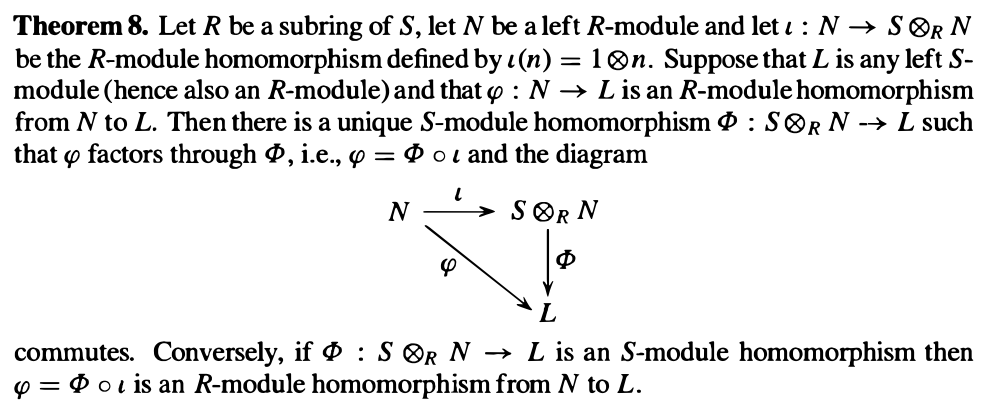
\includegraphics[width=\textwidth]{tensor-product-2025050211.png}
% \caption{}
\label{}
\end{figure}
\end{definition}
\begin{example}
\begin{figure}[H]
\centering
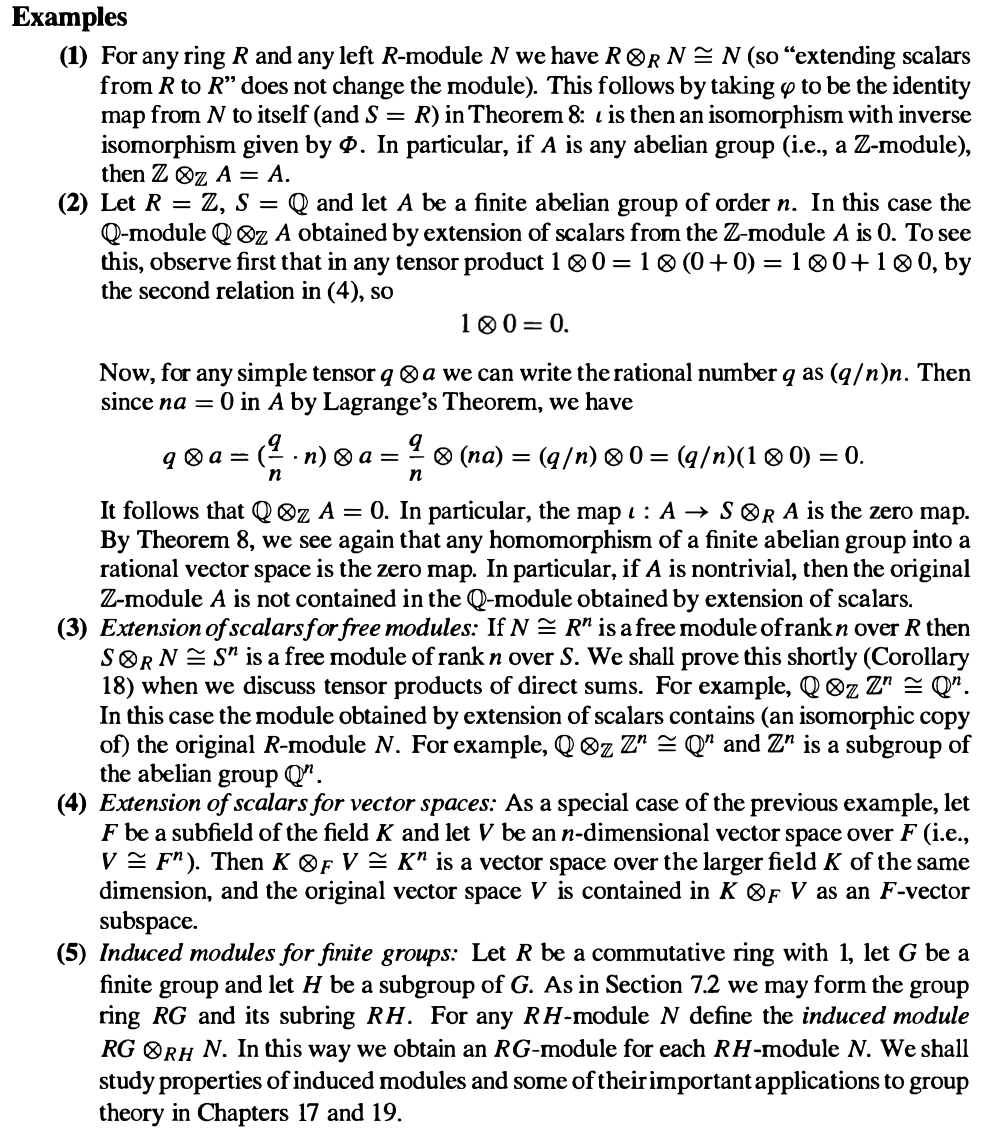
\includegraphics[width=\textwidth]{1-tensor-product-2025050211.png}
% \caption{}
\label{}
\end{figure}
\end{example}
\begin{definition}[$R$ -balanced]
\begin{figure}[H]
\centering
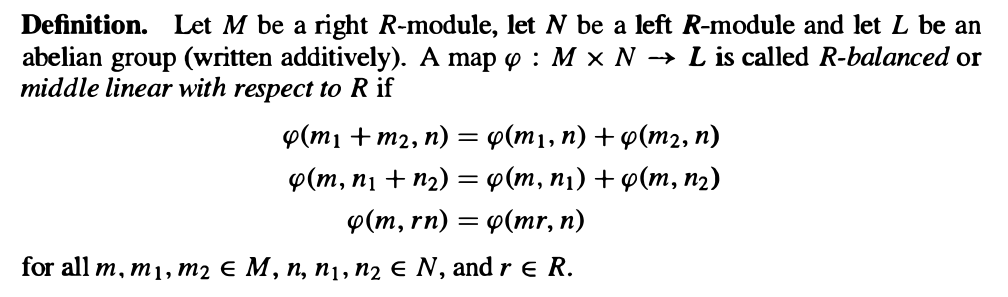
\includegraphics[width=\textwidth]{tensor-product-2025050214.png}
% \caption{}
\label{}
\end{figure}
\end{definition}
\begin{definition}[$R$ -bilinear]
\begin{figure}[H]
\centering
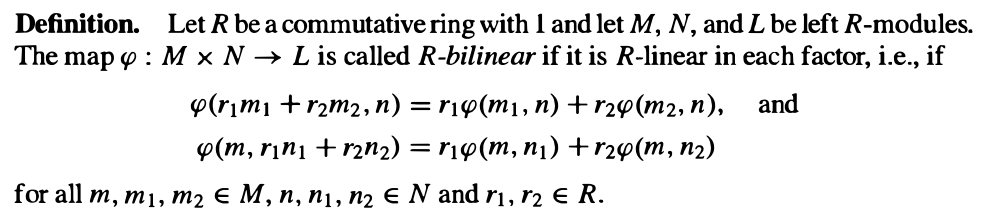
\includegraphics[width=\textwidth]{1-tensor-product-2025050214.png}
% \caption{}
\label{}
\end{figure}
\end{definition}
\begin{example}
We have $\mathbb{Z}_{2}\otimes_{\mathbb{Z}}\mathbb{Z}_{3}=0$, since $3a=a$ for $a\in \mathbb{Z}_{2}$ so that
\[
a\otimes b=3a\otimes b=a\otimes (3b)=a\otimes 0=0
\]
and every simple tensor is reduced to 0. In particular $1\otimes1=0$.
\end{example}
\begin{example}
We have $\mathbb{Z}_{2}\otimes_{\mathbb{Z}}\mathbb{Z}_{2}\cong \mathbb{Z}_{2}$, since $0\otimes0=1\otimes0=0\otimes1=0$ and $1\otimes1$ generates $\mathbb{Z}_{2}\otimes \mathbb{Z}_{2}$.
\end{example}
\begin{example}
$\mathbb{Q}/\mathbb{Z}\otimes_{\mathbb{Z}}\mathbb{Q}/\mathbb{Z}=0$, where a simple tensor has the form $(a/b\ \mathrm{mod}\ \mathbb{Z})\otimes(c/d \ \mathrm{mod}\ \mathbb{Z})$ for some rational numbers $a/b$ and $c/d$. Then
\begin{equation}
\begin{aligned}
\left( \frac{a}{b}\ \mathrm{mod}\ \mathbb{Z} \right)\otimes \left( \frac{c}{d}\ \mathrm{mod}\ \mathbb{Z} \right) & =d\left( \frac{a}{bd}\mod\mathbb{Z} \right)\otimes \left( \frac{c}{d}\mod\mathbb{Z} \right) \\
 & =\left( \frac{a}{bd}\mod\mathbb{Z} \right)\otimes d\left( \frac{c}{d}\mod\mathbb{Z} \right) \\
 & =\left( \frac{a}{bd}\mod\mathbb{Z} \right)\otimes 0 \\
 & =0
\end{aligned}
\label{d2f1db}
\end{equation}
\end{example}

\begin{example}
Similar to \cref{d2f1db}, $A\otimes_{\mathbb{Z}}B=0$ for any divisible abelian group $A$ and \textbf{torsion} abelian group $B$ (an abelian group in which every element has finite order). For exmaple, $\mathbb{Q}\otimes_{\mathbb{Z}}\mathbb{Q}/\mathbb{Z}=0$.
\end{example}
\begin{example}[dimension]
The structure of a tensor product can vary considerably depending on the ring over which the tensors are taken. $\mathbb{Q}\otimes_{\mathbb{Q}}\mathbb{Q}$ and $\mathbb{Q}\otimes_{\mathbb{Z}}\mathbb{Q}$ are isomorphic as left $\mathbb{Q}$ -modules (both are one dimensional vector spaces over $\mathbb{Q}$). Pick any simple tensor $\frac{a}{b}\otimes_{\mathbb{Q}} \frac{c}{d}$ in $\mathbb{Q}\otimes_{\mathbb{Q}}\mathbb{Q}$, then
\[
\frac{a}{b}\otimes \frac{c}{d}=1\otimes \frac{ac}{bd}\to\frac{ac}{bd}
\]
induces an isomorphism between $\mathbb{Q}\otimes_{\mathbb{Q}}\mathbb{Q}$ and $\mathbb{Q}$. Pick any simple tensor $\frac{a}{b}\otimes_{\mathbb{Z}}\frac{c}{d}$ in $\mathbb{Q}\otimes_{\mathbb{Z}}\mathbb{Q}$, then
\[
\frac{a}{b}\otimes \frac{c}{d}=\frac{1}{b}\otimes \frac{ac}{d}=\frac{1}{b}\otimes \left( b\cdot\frac{ac}{bd} \right)=1\otimes \frac{ac}{bd}
\]
Thus $\mathbb{Q}\otimes_{\mathbb{Z}}\mathbb{Q}\cong \mathbb{Q}$. Hence,
\[
\dim _{\mathbb{Q}}(\mathbb{Q}\otimes _{\mathbb{Q}}\mathbb{Q})=\dim _{\mathbb{Q}}(\mathbb{Q}\otimes _{\mathbb{Z}}\mathbb{Q})=1
\]
\end{example}
\begin{example}
On the other hand, $\mathbb{C}\otimes_{\mathbb{C}}\mathbb{C}$ and $\mathbb{C}\otimes_{\mathbb{R}}\mathbb{C}$ are not isomorphic $\mathbb{C}$ -modules (the former is a 1-dimensional vector space over $\mathbb{C}$ and the latter is 2-dimensional over $\mathbb{C}$). Every simple tensor in $\mathbb{C}\otimes_{\mathbb{C}}\mathbb{C}$ has the form $a\otimes b$, then
\[
a\otimes b=1\otimes ab\to ab
\]
induces an isomorphism between $\mathbb{C}\otimes_{\mathbb{C}}\mathbb{C}$ and $\mathbb{C}$. Every simple tensor in $\mathbb{C}\otimes_{\mathbb{R}}\mathbb{C}$ has the form $(a+\mathrm{i}b)\otimes c$, then
\[
(a+\mathrm{i}b)\otimes c=a\otimes c+(\mathrm{i}b)\otimes c=1\otimes (ac)+\mathrm{i}\otimes (bc)\overset{ \simeq  }{ \longrightarrow  }(ac,bc)
\]
induces an isomorphism between $\mathbb{C}\otimes_{\mathbb{R}}\mathbb{C}$ and $\mathbb{C}\oplus \mathbb{C}$. Hence
\[
\dim_{\mathbb{C}} (\mathbb{C}\otimes _{\mathbb{C}}\mathbb{C})=\dim _{\mathbb{C}}\mathbb{C}=1\qquad \dim _{\mathbb{C}}(\mathbb{C}\otimes _{\mathbb{R}}\mathbb{C})=\dim _{\mathbb{C}}(\mathbb{C}\oplus \mathbb{C})=2
\]
\end{example}
\subsection{Dimension}

\href{https://math.stackexchange.com/questions/4306709/dimension-of-a-tensor-product-as-a-vector-space-over-complex-number-field-math}{abstract algebra - Dimension of a tensor product as a vector space over complex number field $\mathbb{C}$ - Mathematics Stack Exchange}

\begin{exercise}
Problem 2 (10 points). Consider the polynomial ring $A=\mathbb{C}[x]$ and its subring $B=\mathbb{C}\left[x^2\right] \subset A$.
Consider $A$ -modules
\[
M=\mathbb{C}[x] /\left(x^2+x\right), \quad N=\mathbb{C}[x] /\left(x^2-1\right)
\]What is the dimension as $\mathbb{C}$ -vector space of each tensor product below? No need to prove or explain.
\end{exercise}
(a) $M \otimes_{\mathbb{C}} N$;

$\mathbb{C}[x]/(x^2+x)\otimes_{\mathbb{C}}\mathbb{C}[x]/(x^2-1)$ has every simple tensor of the form $(a+bx)\otimes_{\mathbb{C}}(c+dx )$, then
\[
\begin{aligned}
(a+bx)\otimes (c+dx ) & =a\otimes c+bx\otimes c+a\otimes dx+bx\otimes dx \\
 & =1\otimes (ac)+x\otimes (bc)+(ad)\otimes x+bd(x\otimes x) \\
 & =ac(1\otimes 1)+bc(x\otimes 1)+ad(1\otimes x)+bd(x\otimes x) \\
 & \to(ac,bc,ad,bd)
\end{aligned}
\]
induces an isomorphism between $\mathbb{C}[x]/(x^2+x)\otimes_{\mathbb{C}}\mathbb{C}[x]/(x^2-1)$ and $\mathbb{C}^{4}$ (the construction is left as an exercise). Therefore
\[
\dim _{\mathbb{C}}(M\otimes _{\mathbb{C}}N)=\dim _{\mathbb{C}}(\mathbb{C}^{4})=4
\]
(b) $M \otimes_A N$;

$\mathbb{C}[x]/(x^2+x)\otimes_{\mathbb{C}[x]}\mathbb{C}[x]/(x^2-1)$ has every simple tensor of the form $(a+bx)\otimes_{\mathbb{C}[x]}(c+dx )$, then
\[
\begin{aligned}
(a+bx)\otimes (c+dx ) & =ac(1\otimes 1)+bc(x\otimes 1)+ad(1\otimes x)+bd(x\otimes x) \\
 & =ac(1\otimes 1)+(bc+ad)((-x^2)\otimes 1)+bd(1\otimes x^2) \\
 & =ac(1\otimes 1)-(bc+ad)(1\otimes x^2)+bd(1\otimes 1) \\
 & =(ac-bc-ad+bd)(1\otimes 1) \\
 & \to ac-bc-ad+bd
\end{aligned}
\]
induces a nature isomorphism between $M\otimes_{A}N$ and $\mathbb{C}$. Therefore,
\[
\dim _{\mathbb{C}}(M\otimes _{A}N)=\dim _{\mathbb{C}}\mathbb{C}=1
\]
(c) $M \otimes_B N$.

$\mathbb{C}[x]/(x^2+x)\otimes_{\mathbb{C}[x^2]}\mathbb{C}[x]/(x^2-1)$ has every simple tensor of the form $(a+bx)\otimes_{\mathbb{C}[x^2]}(c+dx )$, then
\[
\begin{aligned}
(a+bx)\otimes (c+dx  ) & =(a-bx^2)\otimes (c+dx) \\
 & =a\otimes (c+dx )-bx^2\otimes (c+dx) \\
 & =1\otimes (ac+adx)-1\otimes (bcx^2+cdx^3) \\
 & =1\otimes (ac+adx)-1\otimes (bc+cdx) \\
 & =1\otimes [(ac-bc)+(ad-cd)x] \\
 & =(ac-bc)(1\otimes 1)+(ad-cd)(1\otimes x)  \\
 & \to(ac-bc,ad-cd)
\end{aligned}
\]
induces a nature isomorphism between $M\otimes_{B}N$ and $\mathbb{C}^2$. Therefore,
\[
\dim _{\mathbb{C}}(M\otimes _{B}N)=\dim _{\mathbb{C}}(\mathbb{C}^2)=2
\]
We are done!
